\documentclass[tikz,border=5pt]{standalone}
\usepackage{fontspec}
\setmainfont{Times New Roman}
\usepackage{unicode-math}
\setmathfont{Cambria Math}
\usetikzlibrary{shapes.geometric,positioning,fit,backgrounds,arrows.meta,calc}

\begin{document}
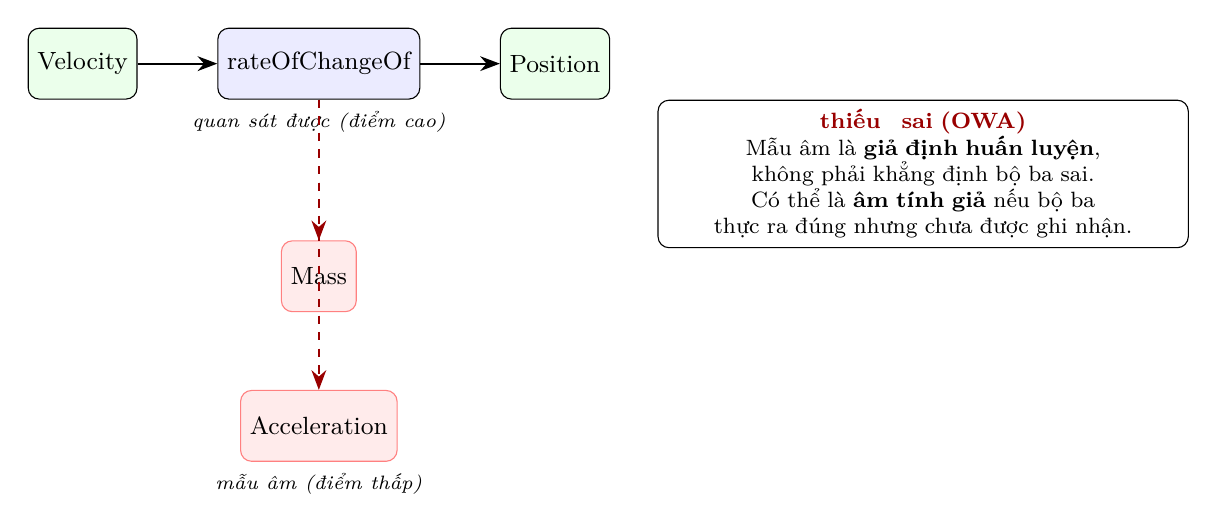
\begin{tikzpicture}[
  ent/.style={rectangle, draw, rounded corners, align=center, minimum height=0.9cm, font=\small},
  arrow/.style={-{Stealth[length=2.5mm]}, thick},
  label/.style={font=\scriptsize\itshape},
]

% === Positive triple ===
\node[ent, fill=green!8] (h) at (0, 2.0) {Velocity};
\node[ent, fill=blue!8] (r) at (3.0, 2.0) {rateOfChangeOf};
\node[ent, fill=green!8] (t) at (6.0, 2.0) {Position};
\draw[arrow] (h) -- (r);
\draw[arrow] (r) -- (t);
\node[label, below=0.02cm of r] {quan sát được (điểm cao)};

% === Corruptions ===
\node[ent, fill=red!8, draw=red!50] (n1) at (3.0, -0.7) {Mass};
\node[ent, fill=red!8, draw=red!50] (n2) at (3.0, -2.6) {Acceleration};

\draw[arrow, dashed, red!60!black] (r) -- (n1);
\draw[arrow, dashed, red!60!black] (r) -- (n2);

\node[label, below=0.02cm of n2] {mẫu âm (điểm thấp)};

% === Annotation ===
\node[draw, rounded corners, align=center, font=\footnotesize, text width=6.5cm, right=0.6cm of t.south east, anchor=north west]
  (ann) {%
    \textcolor{red!60!black}{\textbf{thiếu ≠ sai (OWA)}}\\
    Mẫu âm là \textbf{giả định huấn luyện},\\
    không phải khẳng định bộ ba sai.\\
    Có thể là \textbf{âm tính giả} nếu bộ ba\\
    thực ra đúng nhưng chưa được ghi nhận.
};

\end{tikzpicture}
\end{document}